\documentclass[11pt,fontset=fandol]{ctexart}

\usepackage[a4paper, margin=1in]{geometry}
\usepackage{amsmath}
\usepackage{graphicx}
\usepackage{booktabs}
\usepackage{hyperref}

\title{Project 1 Report Notes}
\author{姓名：于翔 \quad 学号：23307130202}
\date{\today}

\begin{document}
\maketitle

\section{MLP Baseline}

本节记录 Part A 的实现与实验结果。按照项目要求，本部分只完成 MLP baseline，不引入 CNN、momentum、learning rate scheduler、L2 regularization、dropout 等后续比较项，避免基线设置与 Part B/Part C 混淆。

\subsection{Implementation}

本部分主要修改了以下文件：

\begin{itemize}
    \item \texttt{codes/mynn/op.py}: 实现 \texttt{Linear.forward}、\texttt{Linear.backward} 和 \texttt{MultiCrossEntropyLoss}。
    \item \texttt{codes/mynn/models.py}: 修正 \texttt{Model\_MLP} 的初始化与模型加载逻辑。
    \item \texttt{codes/mynn/optimizer.py}: 修正 \texttt{SGD.step}，使用原地参数更新，确保 \texttt{Linear.forward} 中实际使用的 \texttt{W} 和 \texttt{b} 被更新。
    \item \texttt{codes/mynn/runner.py}: 修正训练循环中的空 batch 问题，并将验证改为按固定间隔执行。
    \item \texttt{codes/test\_train.py}: 设置并运行 MLP baseline 训练流程。
    \item \texttt{codes/test\_model.py}: 加载保存的 baseline 模型并在测试集上评估。
\end{itemize}

线性层前向传播为
\[
    Y = XW + b.
\]
反向传播中，设下一层传回梯度为 \(\frac{\partial L}{\partial Y}\)，则
\[
    \frac{\partial L}{\partial W} = X^\top \frac{\partial L}{\partial Y},
    \quad
    \frac{\partial L}{\partial b} = \sum_i \frac{\partial L}{\partial Y_i},
    \quad
    \frac{\partial L}{\partial X} = \frac{\partial L}{\partial Y} W^\top.
\]

分类损失采用 softmax cross entropy。实现中先对 logits 做数值稳定的 softmax，再计算平均交叉熵损失。反向传播使用 softmax 与 cross entropy 合并后的梯度：
\[
    \frac{\partial L}{\partial z} = \frac{p - y}{N},
\]
其中 \(p\) 为 softmax 概率，\(y\) 为 one-hot 标签，\(N\) 为 batch size。

\subsection{Training Setting}

MNIST 训练集共 60000 张图像。实验中固定随机种子为 309，将其中 10000 张作为 validation set，其余 50000 张作为 training set。输入图像展平为 784 维向量，并归一化到 \([0, 1]\)。

\begin{table}[h]
\centering
\begin{tabular}{ll}
\toprule
Item & Setting \\
\midrule
Model & MLP \\
Architecture & \(784 \rightarrow 256 \rightarrow 10\) \\
Activation & ReLU \\
Loss & Softmax cross entropy \\
Optimizer & SGD \\
Learning rate & 0.1 \\
Batch size & 128 \\
Epochs & 5 \\
Validation size & 10000 \\
\bottomrule
\end{tabular}
\caption{Part A MLP baseline setting.}
\end{table}

\subsection{Results}

训练完成后，保存的最佳模型位于
\texttt{codes/best\_models/mlp/best\_model.pickle}。学习曲线保存于
\texttt{codes/figs/part\_a\_mlp\_learning\_curve.png}。

\begin{table}[h]
\centering
\begin{tabular}{lc}
\toprule
Metric & Accuracy \\
\midrule
Best validation accuracy & 0.95240 \\
Test accuracy & 0.95590 \\
\bottomrule
\end{tabular}
\caption{Part A MLP baseline results.}
\end{table}

\begin{figure}[h]
\centering
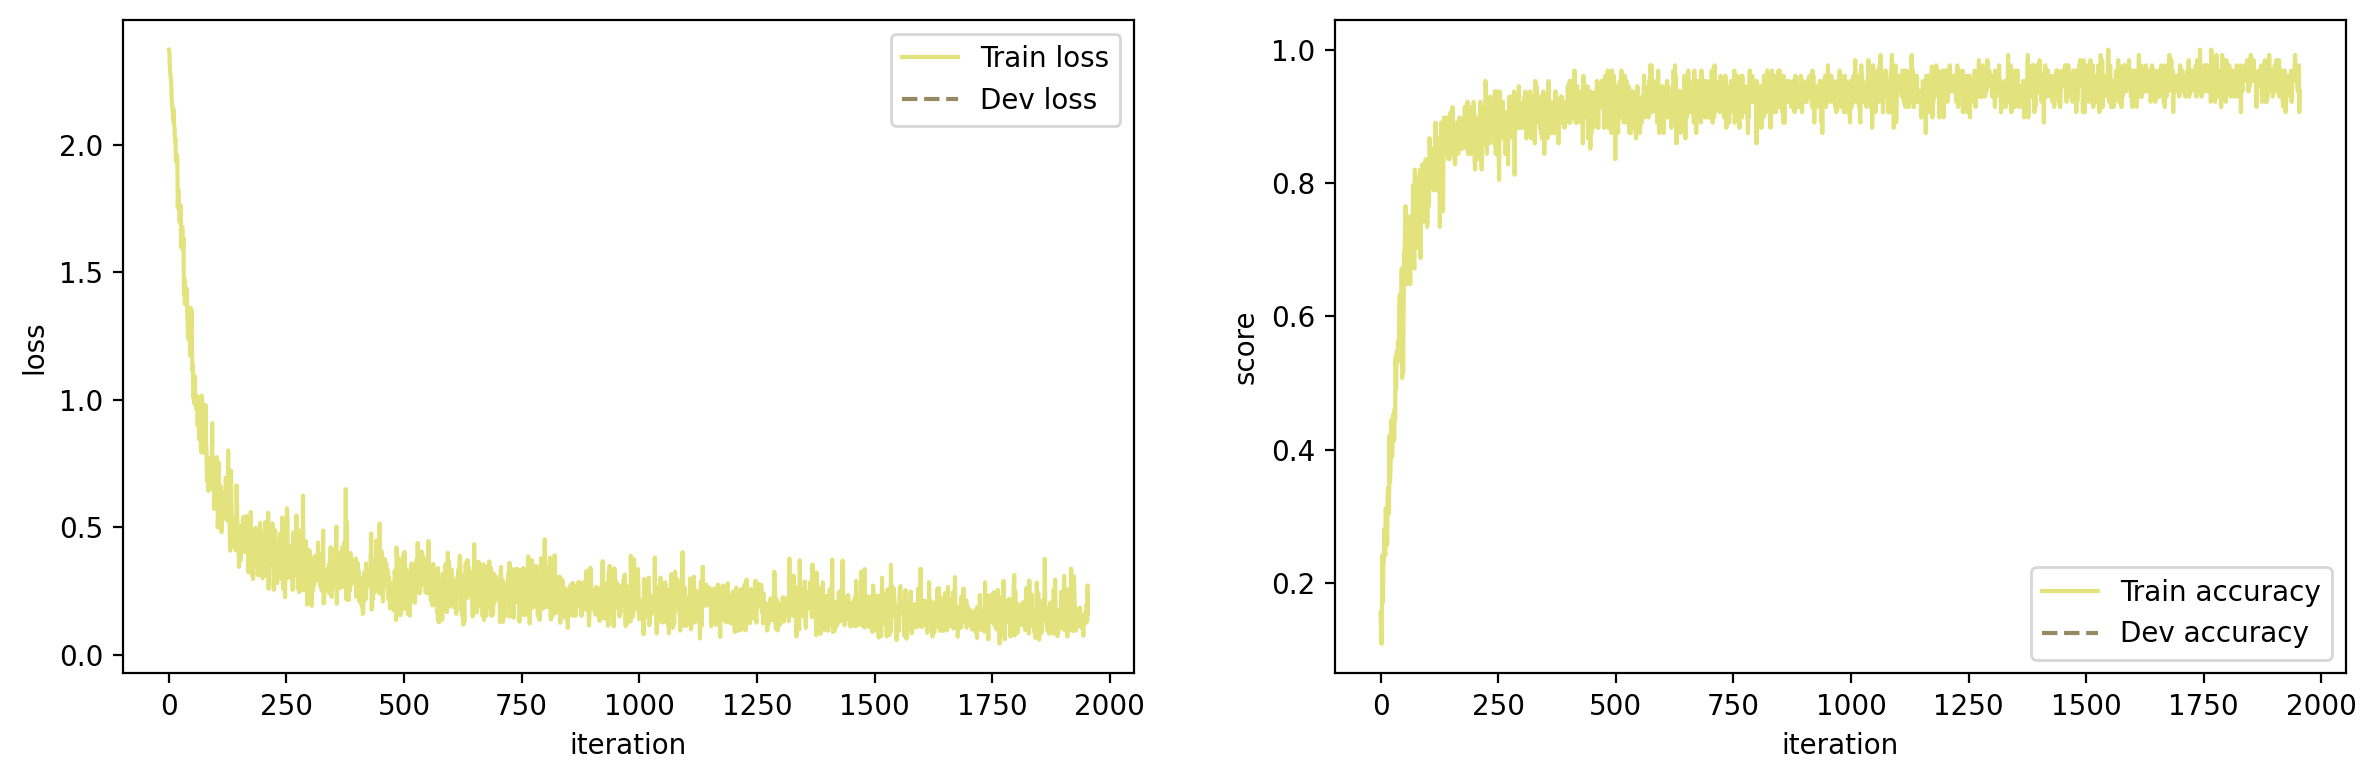
\includegraphics[width=0.85\linewidth]{../codes/figs/part_a_mlp_learning_curve.png}
\caption{Learning curve of the MLP baseline.}
\end{figure}

\section{CNN Model and MLP-vs-CNN Comparison}

本节记录 Part B 的实现与实验结果。按照项目要求，本部分手动实现 \texttt{conv2D}，并基于该算子构建一个简单 CNN，在相近训练设置下与 Part A 的 MLP baseline 进行比较。

\subsection{Implementation}

本部分主要修改或新增了以下文件：

\begin{itemize}
    \item \texttt{codes/mynn/op.py}: 实现 \texttt{conv2D.forward} 和 \texttt{conv2D.backward}，并新增 \texttt{Flatten} 层。
    \item \texttt{codes/mynn/models.py}: 实现 \texttt{Model\_CNN}，包括前向传播、反向传播、模型保存与加载。
    \item \texttt{codes/mynn/runner.py}: 支持按 batch 分批验证，避免 CNN 在验证集上一次性缓存过大的 feature map。
    \item \texttt{codes/test\_train.py}: 通过参数 \texttt{--model cnn} 训练 CNN 模型并保存学习曲线。
    \item \texttt{codes/test\_model.py}: 通过参数 \texttt{--model cnn} 加载保存的 CNN 模型并在测试集上评估。
\end{itemize}

\texttt{conv2D} 的输入为 \([N, C, H, W]\)，卷积核为 \([O, C, K, K]\)。实现中使用 NumPy 的滑动窗口视图构造局部感受野，并使用 \texttt{einsum} 完成卷积计算；反向传播中手动计算卷积核梯度、bias 梯度和输入梯度。该实现没有调用任何深度学习框架或高级神经网络算子。

\subsection{CNN Training Setting}

CNN 采用一个较小的结构，便于在 CPU 上完整训练和复现实验：

\[
    \text{Conv}(1 \rightarrow 8, 3 \times 3, \text{padding}=1)
    \rightarrow \text{ReLU}
    \rightarrow \text{Flatten}
    \rightarrow \text{Linear}(8 \times 28 \times 28 \rightarrow 10).
\]

训练集、验证集划分、随机种子、batch size 和 epoch 数均与 MLP baseline 保持一致。CNN 使用固定学习率 SGD，不使用 momentum、learning rate scheduler 或额外正则化。

\begin{table}[h]
\centering
\begin{tabular}{ll}
\toprule
Item & Setting \\
\midrule
Model & CNN \\
Architecture & Conv-ReLU-Flatten-Linear \\
Conv channels & 8 \\
Kernel size & \(3 \times 3\) \\
Padding & 1 \\
Loss & Softmax cross entropy \\
Optimizer & SGD \\
Learning rate & 0.05 \\
Batch size & 128 \\
Epochs & 5 \\
Validation size & 10000 \\
\bottomrule
\end{tabular}
\caption{Part B CNN setting.}
\end{table}

\subsection{Comparison Results}

CNN 训练完成后，保存的最佳模型位于
\texttt{codes/best\_models/cnn/best\_model.pickle}。学习曲线保存于
\texttt{codes/figs/part\_b\_cnn\_learning\_curve.png}。

\begin{table}[h]
\centering
\begin{tabular}{lcc}
\toprule
Model & Best validation accuracy & Test accuracy \\
\midrule
MLP baseline & 0.95240 & 0.95590 \\
CNN & 0.95960 & 0.96130 \\
\bottomrule
\end{tabular}
\caption{MLP-vs-CNN comparison under similar training settings.}
\end{table}

\begin{figure}[h]
\centering
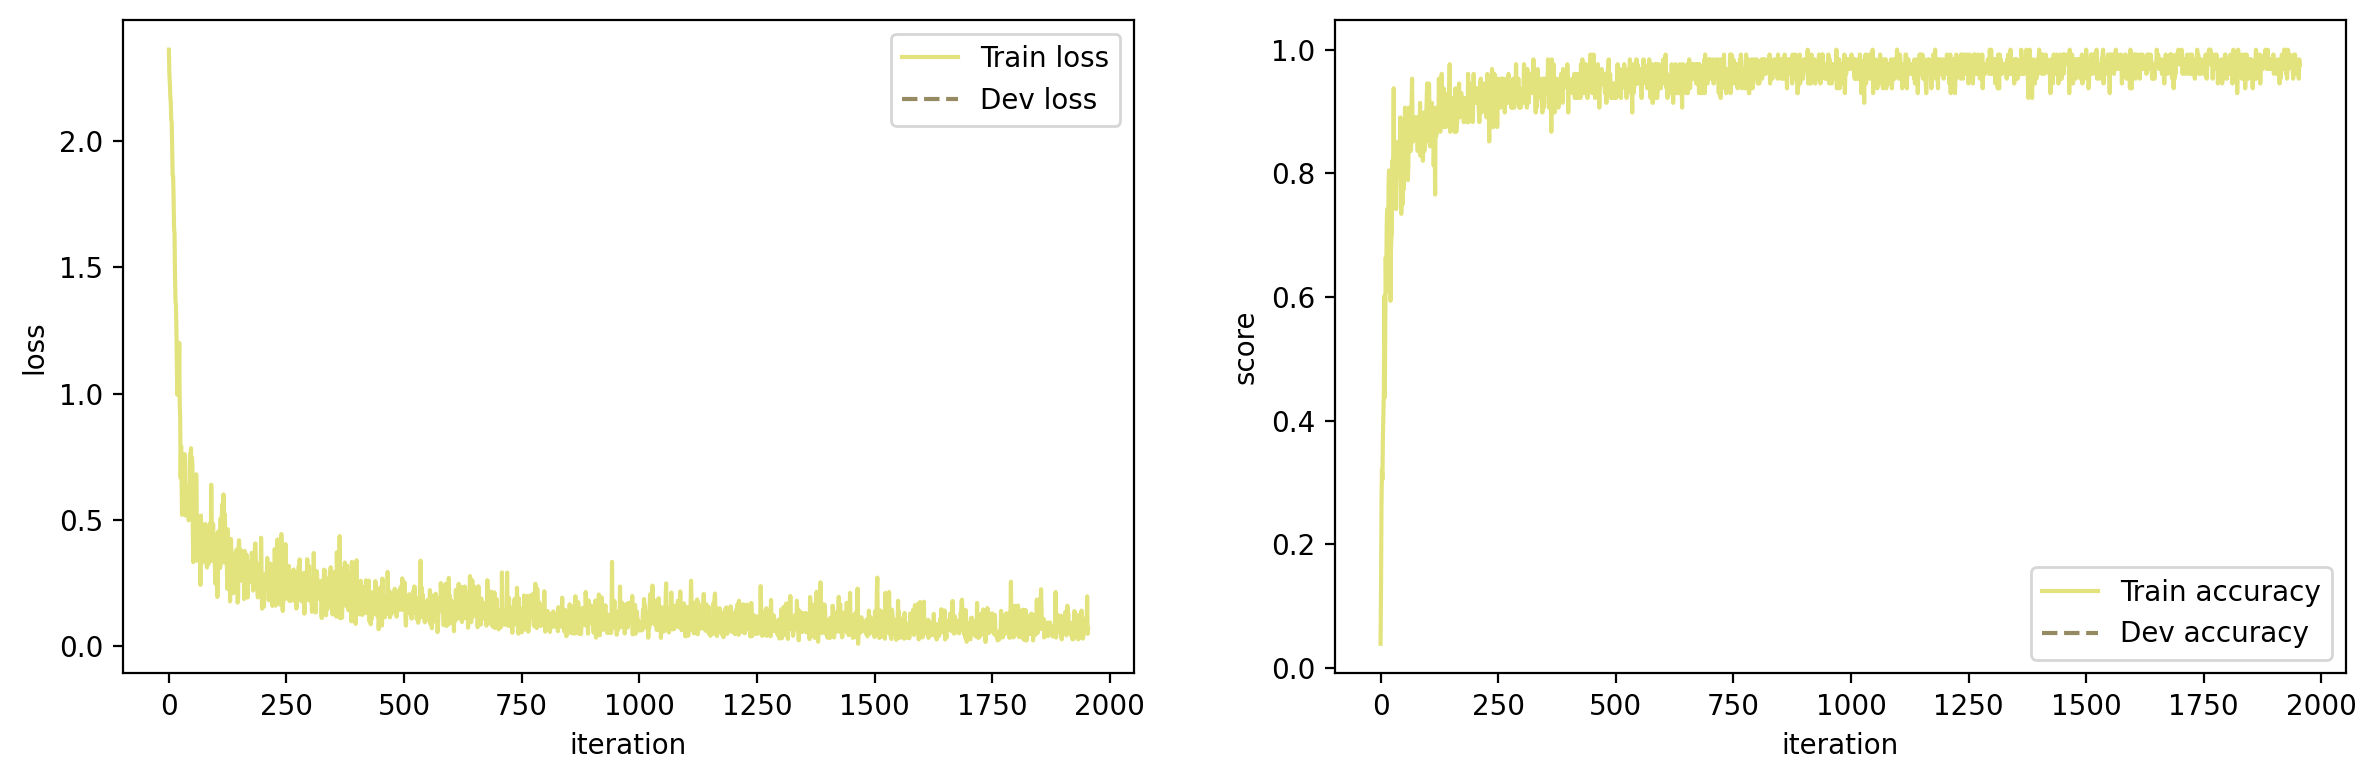
\includegraphics[width=0.85\linewidth]{../codes/figs/part_b_cnn_learning_curve.png}
\caption{Learning curve of the CNN model.}
\end{figure}

\subsection{Discussion}

在当前设置下，CNN 的 validation accuracy 和 test accuracy 都略高于 MLP baseline。主要原因是 CNN 的卷积核共享参数，并利用了图像中的局部空间结构；相比直接把 \(28 \times 28\) 图像展平成向量的 MLP，CNN 更容易学习局部笔画、边缘和小形状等与手写数字相关的模式。

本实验中的 CNN 仍然很简单，只包含一个卷积层，没有使用 pooling、dropout、batch normalization 或更深的卷积结构。因此它的提升幅度有限，但已经体现出卷积模型相对 MLP 更适合图像分类任务的趋势。

\subsection{Current Verification}

已完成以下检查：
\begin{itemize}
    \item \texttt{python3 -m py\_compile} 检查通过。
    \item \texttt{python3 test\_train.py --model mlp} 可完成 MLP 训练并保存模型与学习曲线。
    \item \texttt{python3 test\_model.py --model mlp} 可加载保存模型并输出测试准确率 0.9559。
    \item \texttt{python3 test\_train.py --model cnn} 可完成 CNN 训练并保存模型与学习曲线。
    \item \texttt{python3 test\_model.py --model cnn} 可加载保存 CNN 模型并输出测试准确率 0.9613。
    \item 对 \texttt{conv2D.backward} 做了小规模数值梯度检查，卷积核梯度相对误差约为 \(1.19 \times 10^{-13}\)。
\end{itemize}

\end{document}
